\chapter{Applikasjon}

Dette kapittelet tar for seg arbeidsgangen i prosjektet, en detaljert arkitekturskisse, og en gjennomgang av all funksjonalitet knyttet til geoprosessering, filbehandling, grensesnitt og brukerveiledning.

\section{Arbeidsgang}

Det første som ble gjort i forbindelse med applikasjonen var å få en forståelse av hva som har blitt gjort tidligere, med tanke på valg av grensesnitt og funksjonalitet. Dette var også med på å få en forståelse av hva som var forventet og hva som ligger i ordene \textit{viktig GIS-funksjonalitet}. Et dokument som inneholdt geoprosseseringsfunksjonalitet og lagbehandlingsfunksjoner ble laget utifra tilgjengelige prosjekter\cite{Johanessen}\cite{Strand}\cite{Eglaaen}\cite{Villanger}\cite{Jakobsen} som lå tilgengelig på nett.

De ulike geoprosesseringsoperasjonene inkluderte blant annet:

\begin{frame}

    \begin{tabular}{p{0.4\textwidth}p{0.5\textwidth}}

        \begin{itemize}
            \item Clip
            \item Buffer
            \item Union
            \item Dissolve
        \end{itemize} &

        \begin{itemize}
            \item Difference
            \item Intersection
            \item Bounding box
            \item Filtering
        \end{itemize}
    \end{tabular}

\end{frame}

Mens typiske lagbehandlingsfunksjoner var:

\begin{frame}

    \begin{tabular}{p{0.4\textwidth}p{0.5\textwidth}}

        \begin{itemize}
            \item Legge til lag
            \item Fjerne lag
            \item Endre navn på lag
            \item Endre farge på navn
        \end{itemize} &

        \begin{itemize}
            \item Vise/skjule lag
            \item Zoome til lag
            \item Laste ned lag
        \end{itemize}
    \end{tabular}

\end{frame}

Etter å ha sjekket at de programmeringsspråkene jeg ønsket å jobbe med hadde støtte for denne typen operasjoner var neste steg å sette opp klient-prosjektet og server-prosjektet. Versjonskontrollsystemet git gir stor fleksibilitet til å prøve og feile, samt holde tidligere versjoner av programmet enkelt tilgjengelig hvis det skulle bli nødvendig å gå tilbake. Begge prosjektene ble knyttet til github, og kildekoden finnes på følgende nettadresser:

\href{https://github.com/torsol/PiG-frontend}{Klient-prosjektet}

\href{https://github.com/torsol/PiG-backend}{Server-prosjektet}

Den neste oppgaven var å få en minimal versjon av klient-programmet til å fungere. Det ble laget et initielt React-program som lastet inn en mapbox-komponent. Se figur \ref{fig:firstmap}. Dette var slik applikasjonen så ut etter den commiten til github 3. september.

\begin{figure}[h]
    \center
    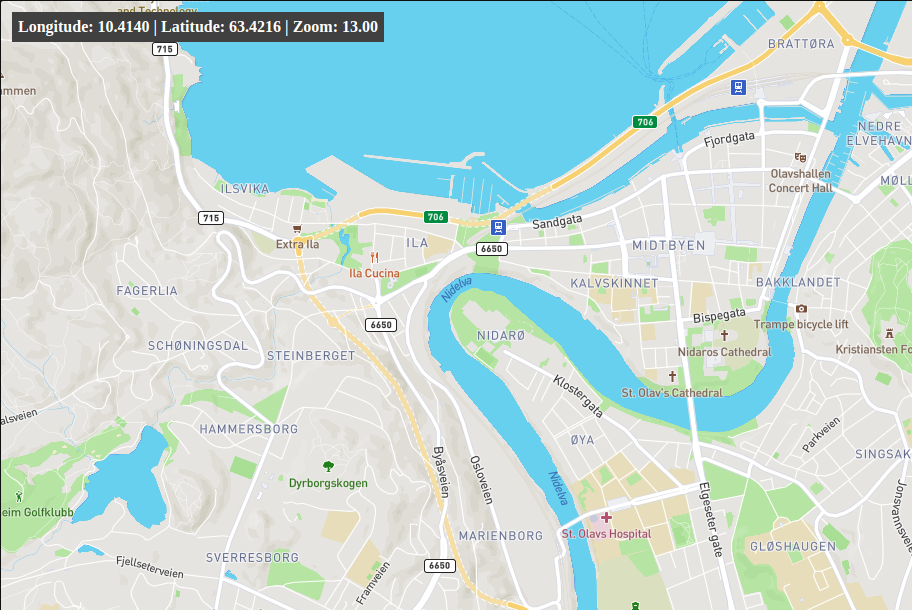
\includegraphics[scale=0.3]{first_frontend.png}
    \caption{Første versjon av klienten}
    \label{fig:firstmap}
\end{figure}

Den neste oppgaven var å få opp Server-prosjektet. Det ble gjort et bevvist valg om å holde programkodene adskilt siden de to applikasjonene i teorien kunne utvikles parallelt. Den aller første kommunikasjonen var et enkelt get-kall til flask-serveren. Som et proof of concept ville et get-kall til '/api/ping' returnere 'pong', see figure \ref{fig:firstping}. Kallet ble gjort via applikasjonen Postman, som er et utviklingsvertkøy for å foreta seg http-kall, dette ble flittig brukt for å teste ulike http-post-kall til serveren gjennom utviklingsprosessen.

\begin{figure}[h]
    \center
    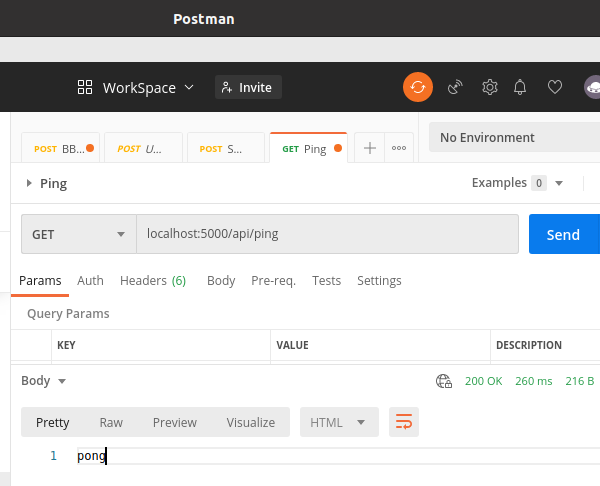
\includegraphics[scale=0.5]{ping.png}
    \caption{Første ping-pong-svar fra server, gjort via Postman}
    \label{fig:firstping}
\end{figure}

Etter at begge prosjektene var oppe og de ulike rammeverkene fungerte isolert, var hovedfokuset på å knytte sammen klient og server, ved å implementere at klienten kunne gjøre egne HTTP-kall for å få data fra serveren. Når også dette fungerte ble det satt opp en løype for å hoste de to tjenestene på github-pages og heroku, slik at man enkelt kunne gjøre nye oppdateringer i applikasjonene tilgjengelig over nett. Mer om dette kommer i seksjon \ref{sec:hosting}.

Når hovedarkitekturen var på plass flyttet fokuset seg over til å implementere mer funksjonalitet og brukergrensesnitt. Funksjonalitet var drevet av de kartlagte funksjonene funnet tidligere i arbeidsprosessen, mens brukergrensesnittet ble laget inspirert av målene om at applikasjonen skulle være brukervennlig og at det skulle bestå av mest mulig interaksjon i kartet.

Videre ble det forberedt data og laget en brukerveiledning som kan finnes både inne i klienten, men også i denne rapporten i appendiks \ref{sec:brukerveiledning}. Helt tilslutt gjenstod det å oppsummere arbeidet i denne rapporten og lansere den endelige versjonen.

\section{Detaljert arkitektur}

Klienten er bygget på React, og følger konvensjonene for bruk av komponenter og State-behandling. En komponent i React kan enten være en klasse, eller en funksjon, skrevet i javascript. Deres oppgave er å returnere HTML som vises i nettleseren når man besøker nettsiden. Det som avgjør hvilken HTML som returneres er komponentenes interne State (eller tilstand). Komponenter kan sende informasjon til hverandre og returnere andre komponenter, og det er en konvensjon at informasjon kun skal flyte fra foreldre-komponenten til barn-komponenten og ikke motsatt. En total nettside består gjerne av flere komponenter, der hver komponent har et ansvarsområde.

i figur \ref{fig:react-arkitektur} kan man se den totale komponent-strukturen til klienten. Rot-komponenten App består av komponentene Sidebar, Map og Tutorial. I tillegg har App ansvaret for State til alle kartlagene som legges til. Sidebar-komponenten har hovedansvaret for å vise sidebaren, og består av komponentene Dropzone, Operation og Layerbar. Dropzone er komponenten som behandler filopplastinger. Layerbar er den delen av sidebaren som viser kartlagene som er lagt til. Operation-komponenten er koblet til APIConnection, som har ansvaret for å kjøre HTTP-forespørsler til Serveren, der den faktiske geoprosesseringen i applikasjonen finner sted. Map-komponenten består av et Mapbox GL JS-map som viser kartlag. Tutorial-komponenten er en egen komponent som har ansvaret for å vise instruksjoner.

Komponentene Dropzone, Operation, LayerBar og Map kan alle (på ulikt vis) manipulere datalagene i kartet, men de oppdaterer ikke sin egen tilstand. Flyten er at de oppdaterer tilstanden til App, også flyter endringen neddover komponent-treet til alle de komponentene som er avhengig av endringen. På denne måten finnes det kun en kilde til sannhet i applikasjonen, man unngår problemet med lokale endringer i en komponent som ikke plukkes opp av en annen komponent.

\begin{figure}[h]
    \center
    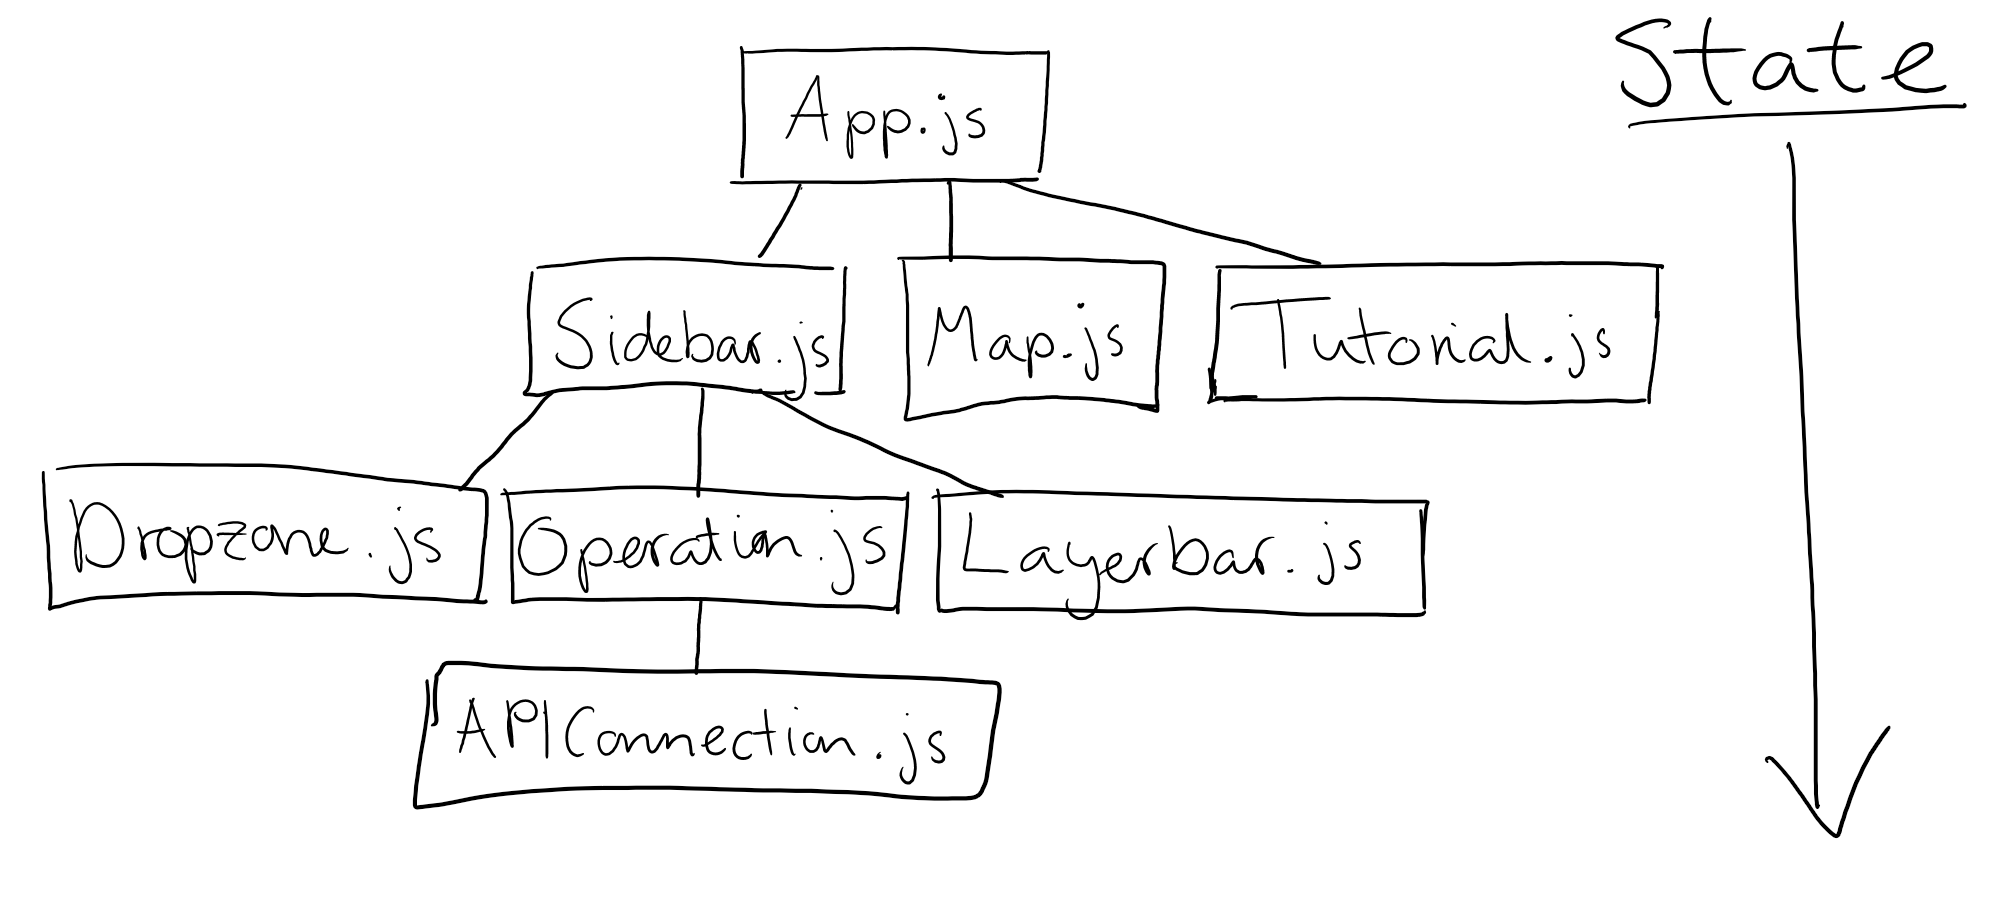
\includegraphics[scale=0.5]{react-arkitektur.PNG}
    \caption{Komponent-diagrammet som viser arv i React-Klienten.}
    \label{fig:react-arkitektur}
\end{figure}

Startpunktet til Serveren er gis\_api.py som importerer app-modulen i prosjektstrukturen. Vanligvis består FLASK-applikasjoner av flere moduler enn api, men i vårt tilfelle importerer app-modulen utelukkende api-modulen. Inne i api-modulen finnes det tre filer som har hovedansvaret for funksjonalitet. Arkitekturen kan sees i figur \ref{fig:api-arktitektur}.

routes.py definerer alle HTTP-endepunktene som serveren skal lytte på og svare på. Hvert endepunkt defineres som en funksjon med såkalte \textit{decorators}, som spesifiserer hvilken URL og HTTP-forespørselstype (GET, PUT, POST, DELETE) som skal matche for å kjøres. Et eksempel er ping-pong-funksjonaliteten nevnt tidligere i prosjektet, se figur \ref{fig:ping-pong}. Alle geoproseseringsoperasjonene har hvert sitt endepunkt, som 'api/buffer' eller 'api/dissolve'.

\begin{figure}[h]
    \center
    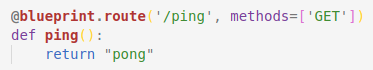
\includegraphics[scale=0.7]{ping-pong-code.png}
    \caption{Eksempel på definisjon av HTTP-endepunkt}
    \label{fig:ping-pong}
\end{figure}



\begin{figure}[h]
    \center
    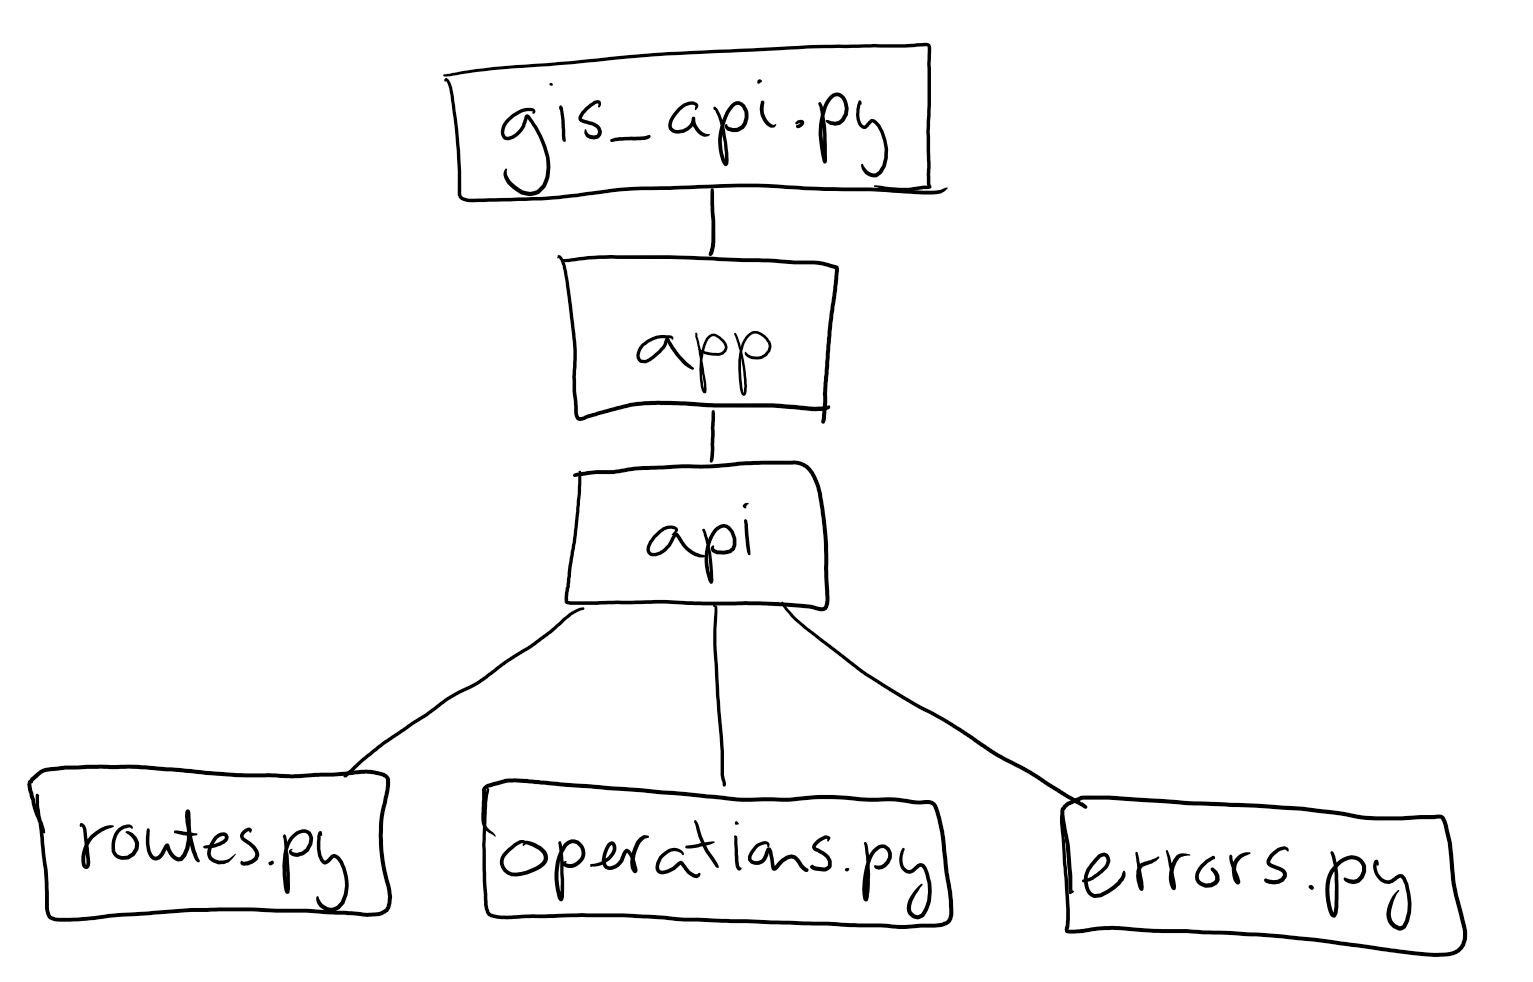
\includegraphics[scale=0.5]{api-arkitektur.PNG}
    \caption{Komponent-diagrammet som viser arv i Python-API'et.}
    \label{fig:api-arktitektur}
\end{figure}

Klienten sender kartdata som en POST-forespørsel til de ulike endepunktene definert i serveren. Endepunktene sender data videre til operations.py, der hver geoprosseringsfunksjon er implementert ved bruk av geopandas. Resultatet sendes tilbake som en respons på HTTP-forespørselen. I tilfelle en feil skjer under utførelsen av HTTP-forespørselen sendes det til errors.py som har ansvaret for å sende tilbake en skreddersydd respons basert på hva som gikk galt. Skreddersydde responser var dessverre ikke mulig å implementere fullstendig. 

Figur \ref{fig:forespørsel} viser flyten når man skal beregne buffer på et kartlag. Klienten gjør klar et HTTP-POST-kall til serveren med riktig endepunkt, buffer-verdi og kartlag. Serveren tar imot forespørselen og beregner bufferen, før den returnerer resultatet til klienten. Det siste klienten gjør er å legge til det nye laget i State og visualisere det i kartet. Denne flyten er representabel for resten av operasjonene i applikasjonen.  

\begin{figure}[h]
    \center
    \includegraphics[scale=0.5]{eksempel-forespørsel.PNG}
    \caption{Flyten mellom Klient og Server for å beregne 100m buffer på en sirkel}
    \label{fig:forespørsel}
\end{figure}

\section{Funksjonalitet}



\subsection{Brukergrensesnitt}

- Tilbakemelding på feil eller suksess

- Design

- Minst mulig sidemenyer

- Kartdesign

\subsection{Geoprosessering}

\subsection{Lagbehandling}

\subsection{Brukerveiledning}

\subsection{Dokumentasjon}

\section{Hosting}
\label{sec:hosting}
